\section{完整数据模拟：政府工作人员的成品报表演示}
\subsection{演示对象、已知资料与数据构造}
为展示资料齐备后的产品输出，程序构造一个虚构的杭州样本社区，含15幢建筑、600户和1500位居民，总建筑面积45000平方米。住户名册按300户2人、300户3人生成；摸排记录含540份问卷和60户补访；分栋协商登记552户同意、30户异议与18户暂缓签署。以上记录统一标记为模拟。真实求是村项目当前的资料导入、结构化事实和完整模型评估仍分别记录；模拟数据通过独立演示视图展示。

建设金额以已归档的广州2024年鸿中楼和青年苑施工合同提供量级参照。两项目的施工合同总价除以总建筑面积分别为308.85和317.78元/平方米。模拟取320元/平方米，45000平方米对应1440万元工程费，拆为基础类800、完善类440、提升类200万元；另加10\%预备费，总预算1584万元。模拟出资为财政1280、居民160、合作方160万元，合计1600万元，预算余额16万元。该设置用于完整报表演示，未实施地区价格指数和具体工程量校准。

\subsection{六维现况怎样生成与比较}
本演示使用可复算的条件覆盖规则：
\[
 q_d=1+4\min\!\left(\frac{a_d}{b_d},1\right),\qquad 1\le q_d\le5.
\]
其中$a_d$为已处理需求、可服务人次、已核对工程任务、支持户数、已明确管护职责或可安排资金，$b_d$为对应的完整数量或预算。当前现况与拟方案使用同一分母，分值保留一位小数。六维名称复用现有注册表；本规则只展示模拟条件覆盖变化，各维的工程和协商安排分别说明。
\begin{center}\small
\begin{tabularx}{\linewidth}{@{}lXXrr@{}}\toprule
维度&模拟现况&拟方案&现况&方案\\\midrule
居民需求&10项诉求处理3项&方案覆盖9项&2.2&4.6\\
公共服务&需求1630人次，可服务920人次&容量2044，服务1630人次&3.3&5.0\\
居住工程&16项接口核对8项&核对15项，剩余公共标识&3.0&4.8\\
实施协同&354/600户支持初始方案&552/600户支持分期方案&3.4&4.7\\
长效维护&10项职责明确5项&10项职责及预算全部登记&3.0&5.0\\
资金交付&1000万元对1584万元预算&1600万元对同一预算&3.5&5.0\\\bottomrule
\end{tabularx}\end{center}

\subsection{完整月度核算与去重人数情景}
模拟核算月份为2026年9月。活动室30席、30场，需求720人次；助餐区40份、26餐，需求832人次；咨询室4名额、26场，需求78人次。三处资源和人员排班分别登记。按既有月度核算接口计算，基准容量2044人次、服务1630人次、去重服务300人，容量利用率79.75\%，居民覆盖率20\%。收费比例依次为0.5、0.9、0.5，单价10、15、20元，单位变动支出2、9、5元；计划收费比例按预算均值登记，模拟台账按完整人次登记。

基准收费收入15612元，其他经营收入5000元，政府购买服务5000元，经营收入合计25612元；固定现金26000元、变动支出9318元，运营现金成本35318元。另记补贴12000元、其他支持0元，支持后现金结余2294元；政府直付场所基础维护2000元，与运营方成本分别列账。财政月投入19000元，政府现金收入设为0。年度预算按本月乘12折算：经营收入30.73万元、运营现金成本42.38万元、政府运营投入22.8万元；居民去重人数仅按月度名册计算。

完整演示为跨情景覆盖率另设月均使用频次模型：$1630/300=5.433333$人次/人。程序先计算容量约束后的服务人次，再除以该频次并四舍五入，以人口和服务人次封顶。需求倍率0.8、1、1.2的结果分别为1304、1630、1956人次，去重人数240、300、360人，覆盖率16\%、20\%、24\%，支持后结余1035、2294、3553元。真实项目模式继续保留未知去重人数，不将此模拟频次外推为实测。

\subsection{模拟月末台账的物理读回}
程序生成1568条模拟服务记录，其中活动684、助餐810、咨询74人次；收费记录分别为342、729、37条，各自按收费单价计费。记录逐条分配至独立场次，每场人数均低于核定容量。活动使用者编号1--180、助餐使用者编号87--286、咨询使用者编号1--74，跨项目去重为286人。台账收费15095元、变动支出9028元，固定现金26500元，运营现金成本35528元；合作收入4800元、购买服务5000元、补贴12000元，支持后现金结余1367元。页面同时展示模拟计划与模拟台账的逐指标差值。

全套数据、600行住户记录、1568行服务台账和Markdown报表均可导出。数值复算沿用现有Python月度核算函数，三个情景全部输出完整指标。模拟数据在独立视图中计算，不写入真实项目事实、实绩或训练样本。
\begin{itemize}
\item 生成源文件：\texttt{packages/retrofit/complete-demo.ts}。
\item 数值复算脚本：\texttt{scripts/build-complete-community-demo.ts}。
\end{itemize}

\subsection{同源数据的交互分析与复合图}
页面首屏提供互动运营推演。用户可连续调整居民需求倍率0.5--1.5、活动室每月15--45场及运营补贴0--20000元；每次调整均调用既有核算接口，先计算容量约束后的服务量，再按模拟使用频次重算去重人数。活动室30席、每场1小时，当前范围内由现有社区岗排班，固定工资预算不变；助餐与咨询排班不变。连续调整会取消旧请求，只有最新输入的完整结果更新画面。用户可在本机保留三个模拟方案并恢复、比较，当前推演的输入与结果同时进入导出。

600户名册、六维现况、标准预算与月末核验按需要展开。名册每格对应一户，点选后显示该栋人口及协商记录；六维前后使用同一刻度。数字、环形进度和资金线条随结果变化，过渡只影响呈现。加载和失败提示由接口返回决定，未完成的调整不会作为当前报表导出。

例如需求调整为150\%、活动15场、补贴0元时，服务1594人次，未满足851人次，去重293人，政府月投入7000元，运营缺口9450元。同样需求下将活动改为45场、补贴12000元，服务2224人次，未满足221人次，去重409人，政府月投入19000元，结余4440元。两项输入和接口结果均已导出读回；固定工资与月均频次沿用上述互动假设。

资金流按金额比例绘制，居民收费、经营收入、政府购买服务和补贴进入运营方账户，政府直付维护另画虚线路径。逐日图从1568条台账按日期汇总，月度去重286人仍由整月居民编号重新计算。报告图采用Nature配色及既有数学建模图的多面板、独立单位和原始记录呈现；网页用较轻的产品配色和操作反馈组织探索。下图为归档样本的三个标准预算情景；互动推演的新增调整另随报表记录输入与结果。

\begin{figure}[htbp]
\centering
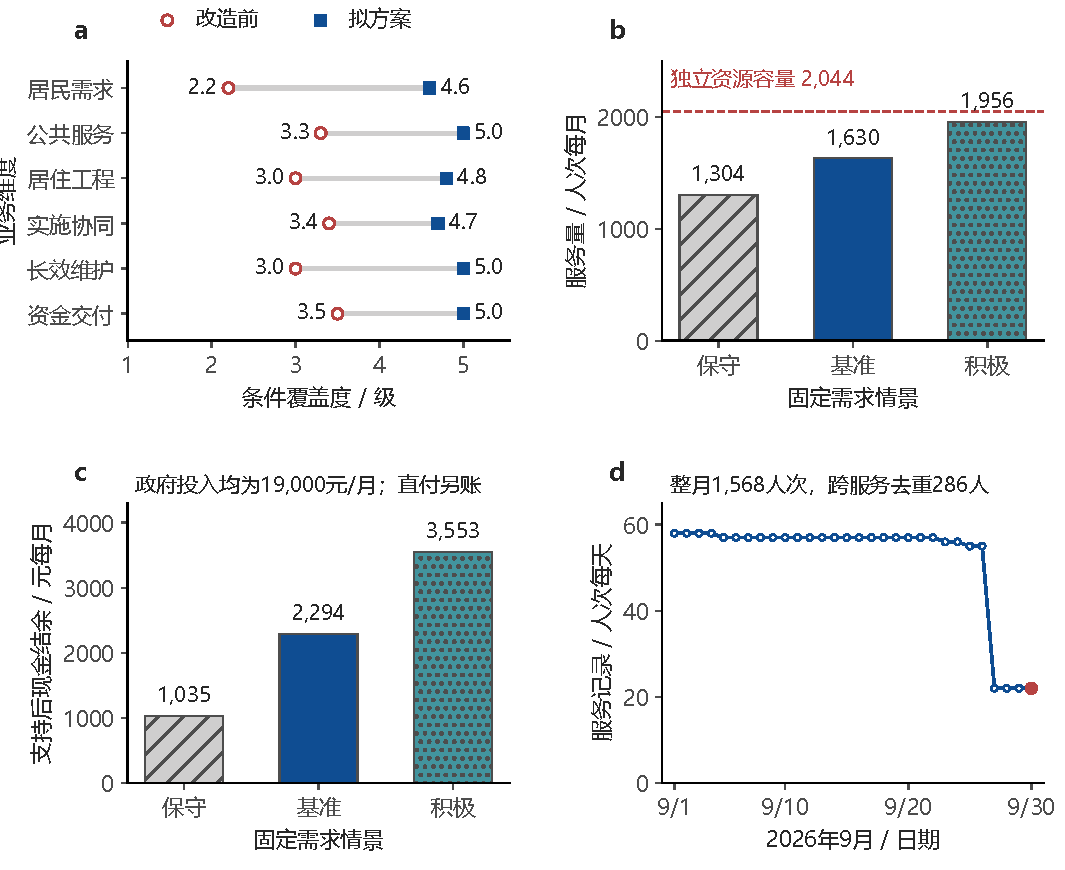
\includegraphics[width=\linewidth]{docs/figures/community-analysis-figure.pdf}
\caption{完整社区模拟数据的四项分析。a：六维现况与拟方案使用同一条件覆盖规则；b：固定需求情景的服务量与2044人次月容量；c：三种情景的支持后运营现金结余，政府直付维护另账；d：1568条模拟台账的逐日服务量。各面板由归档数据直接生成，不包含真实运营效果或统计置信区间。}
\end{figure}
